\documentclass[11pt,a4paper]{article}
\usepackage[utf8]{inputenc}
\usepackage{amsmath}
\usepackage{amsfonts}
\usepackage{amssymb}
\usepackage{graphicx}
\usepackage{hyperref}
\usepackage{geometry}
\usepackage{booktabs}
\usepackage{tabularx}
\usepackage{listings}
\usepackage{xcolor}

\geometry{margin=1in}

\hypersetup{
    colorlinks=true,
    linkcolor=blue,
    filecolor=magenta,      
    urlcolor=cyan,
    pdftitle={MediPilot Implementation README},
}

\title{\textbf{MediPilot Implementation README}\\Architecture, Tech Stack, and Execution}
\author{Team 01 BIT}
\date{\today}

\begin{document}

\maketitle

\begin{abstract}
This document serves as the implementation README, outlining the solution architecture, technology stack, directory structure, synthetic data production, and the specific role of the Large Language Model (LLM). It incorporates the system's architecture diagrams directly to provide a comprehensive, visual guide to the system.
\end{abstract}

\tableofcontents
\newpage

\section{Architectural Implementation \& Tech Stack}

The MediPilot system enforces a strict boundary between perception and evaluation. The architecture is explicitly decoupled to guarantee that clinical risk engines and human interfaces operate in distinct, fail-closed isolation. 

\begin{figure}[ht]
    \centering
    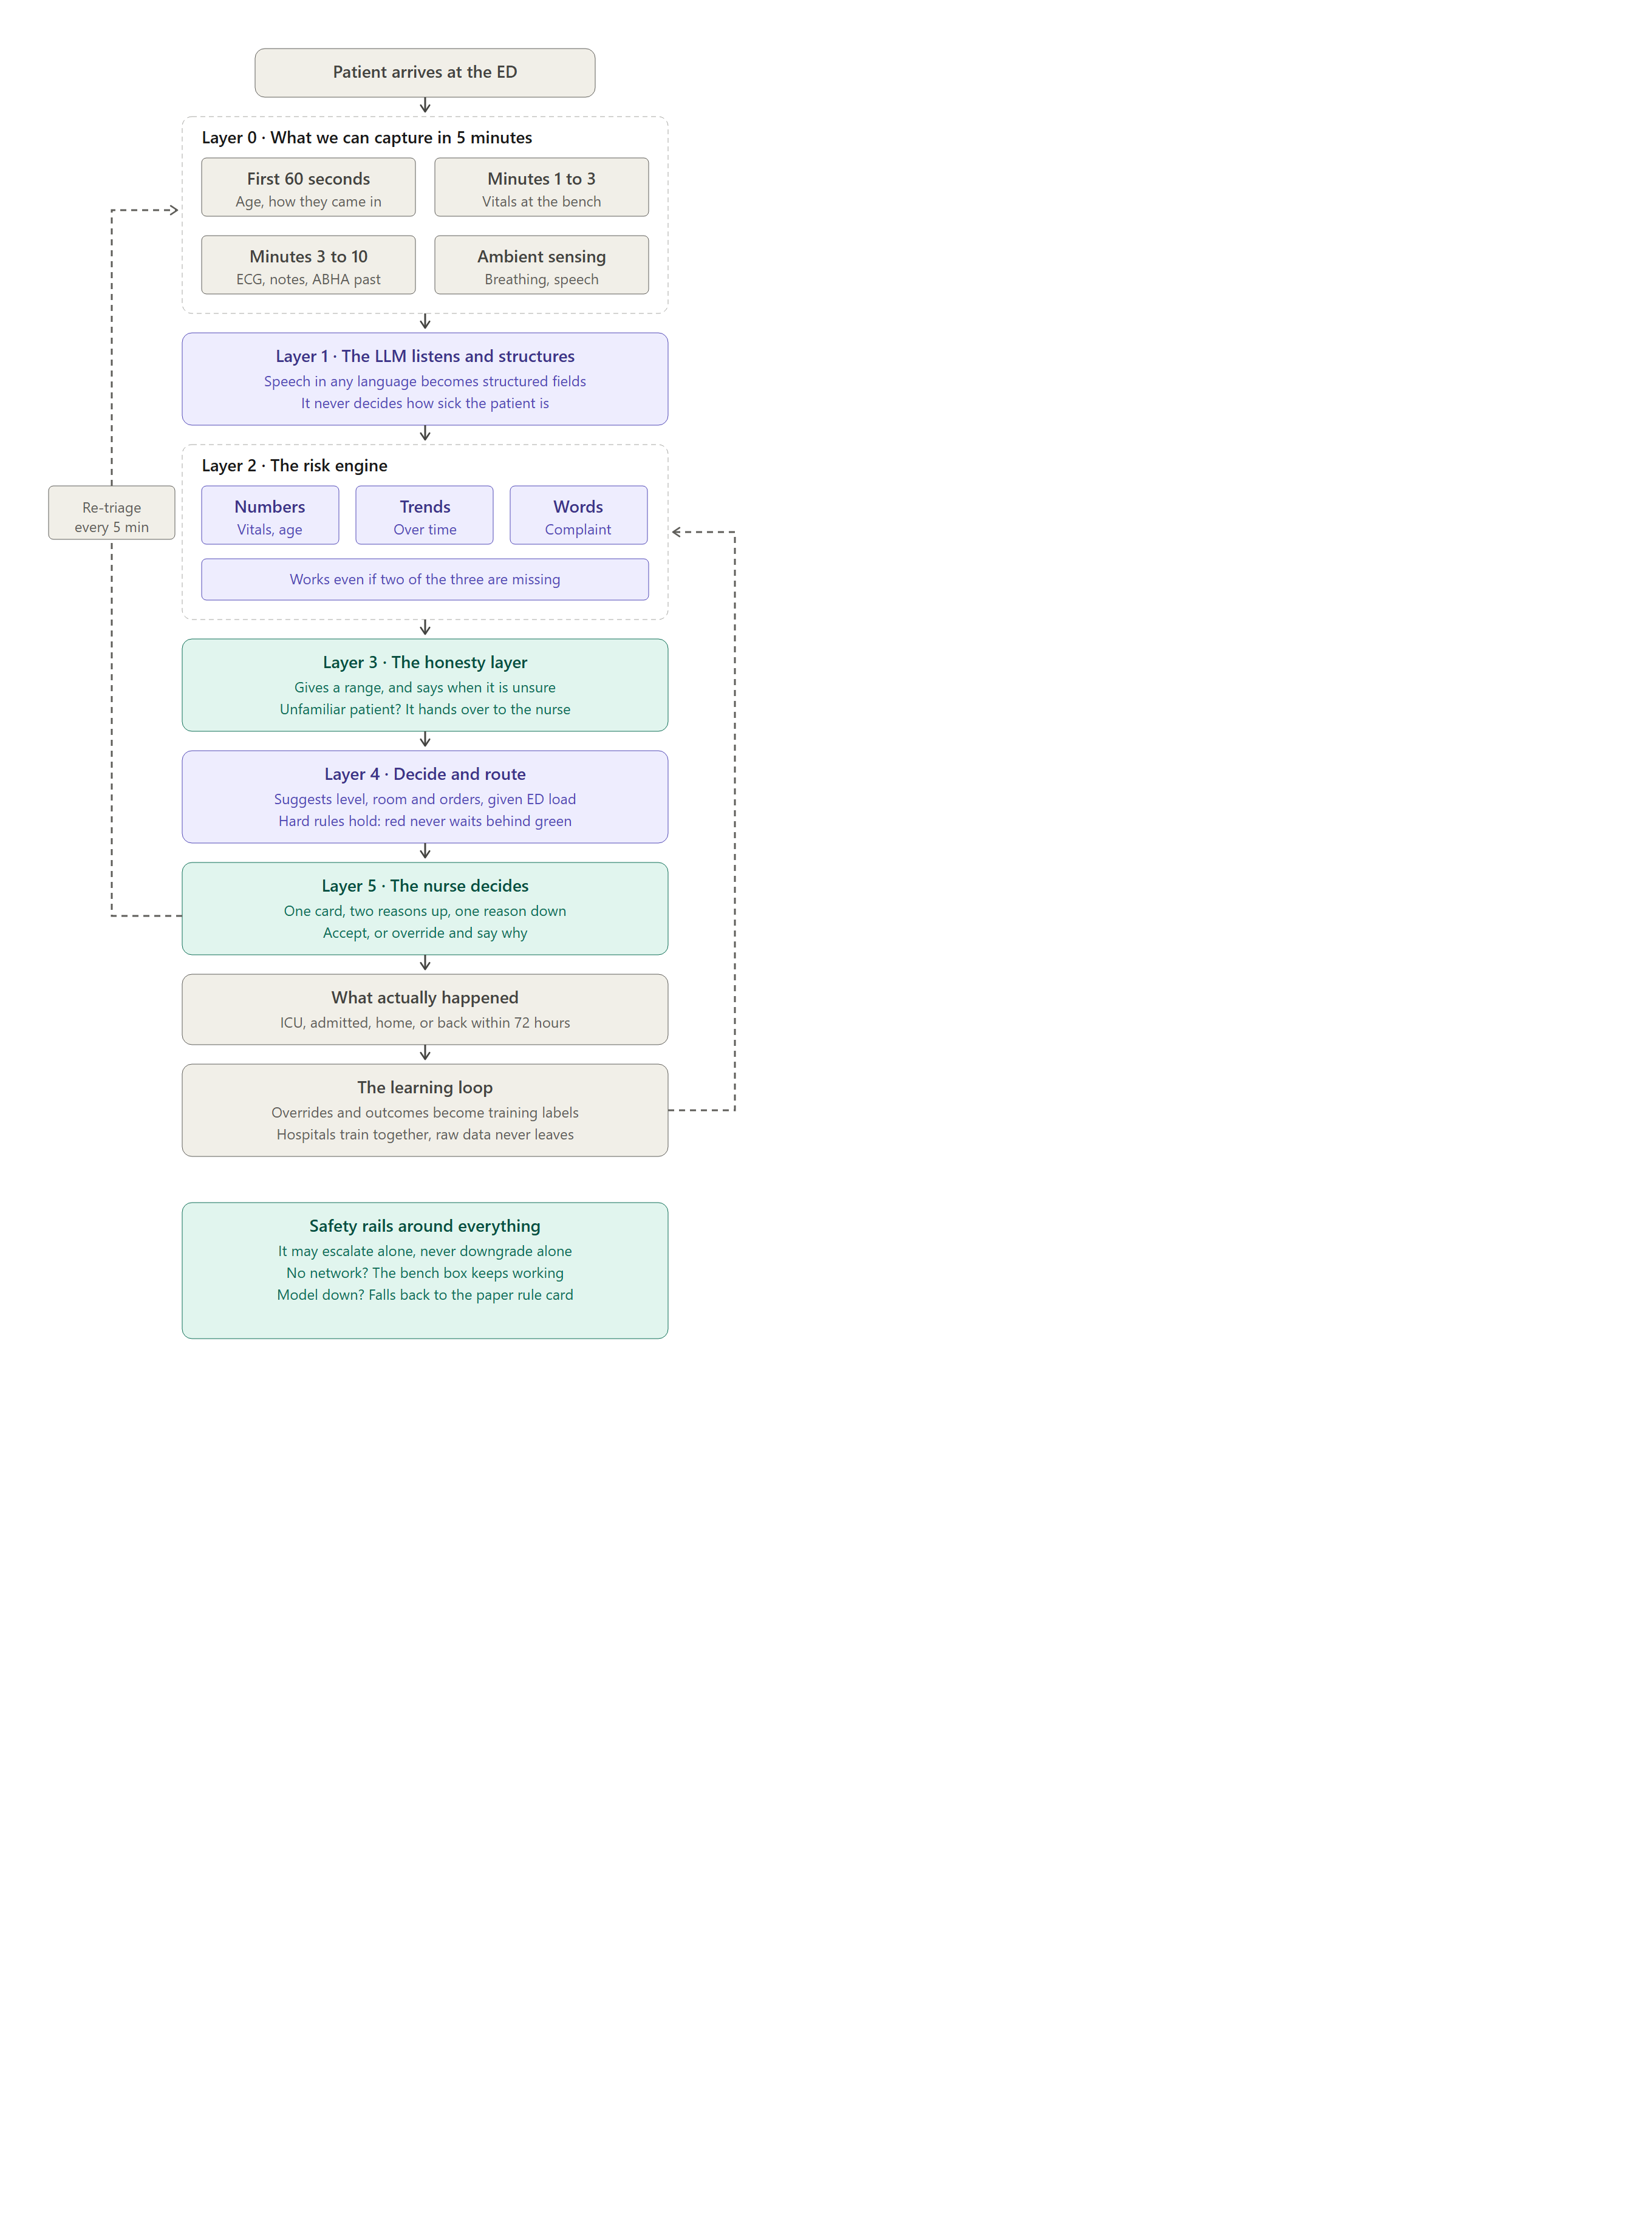
\includegraphics[width=\textwidth]{../diagrams/01-full-architecture.png}
    \caption{The Parallel Track Architecture: Perception (Track A), Interfaces (Track B), and Risk Engine (Track C).}
\end{figure}

\subsection{Track B: The Nurse \& Patient Interfaces (Frontend)}
The interface tier, located in \texttt{web/}, is a static Next.js 16 payload compiled to run as a pure client-side application. It comprises the seven clinical surfaces, including the interactive kiosk and the nurse board. This layer is entirely stripped of clinical authority. It manages the deterministic state machine of the branching triage conversation, raw speech-to-text integration, and local offline phrase matching. It cannot, by construction, evaluate risk.

\subsection{Track C: The Triage Engine (Backend)}
The backend, located in \texttt{backend/}, operates as a Python/FastAPI orchestrator. It receives structured records from the interface tier and evaluates them against a strict hierarchy of safety constraints. The orchestrator houses the deterministic Band Engine, the GBDT Risk Model, and the rigorous age stratification floors. 

\begin{figure}[ht]
    \centering
    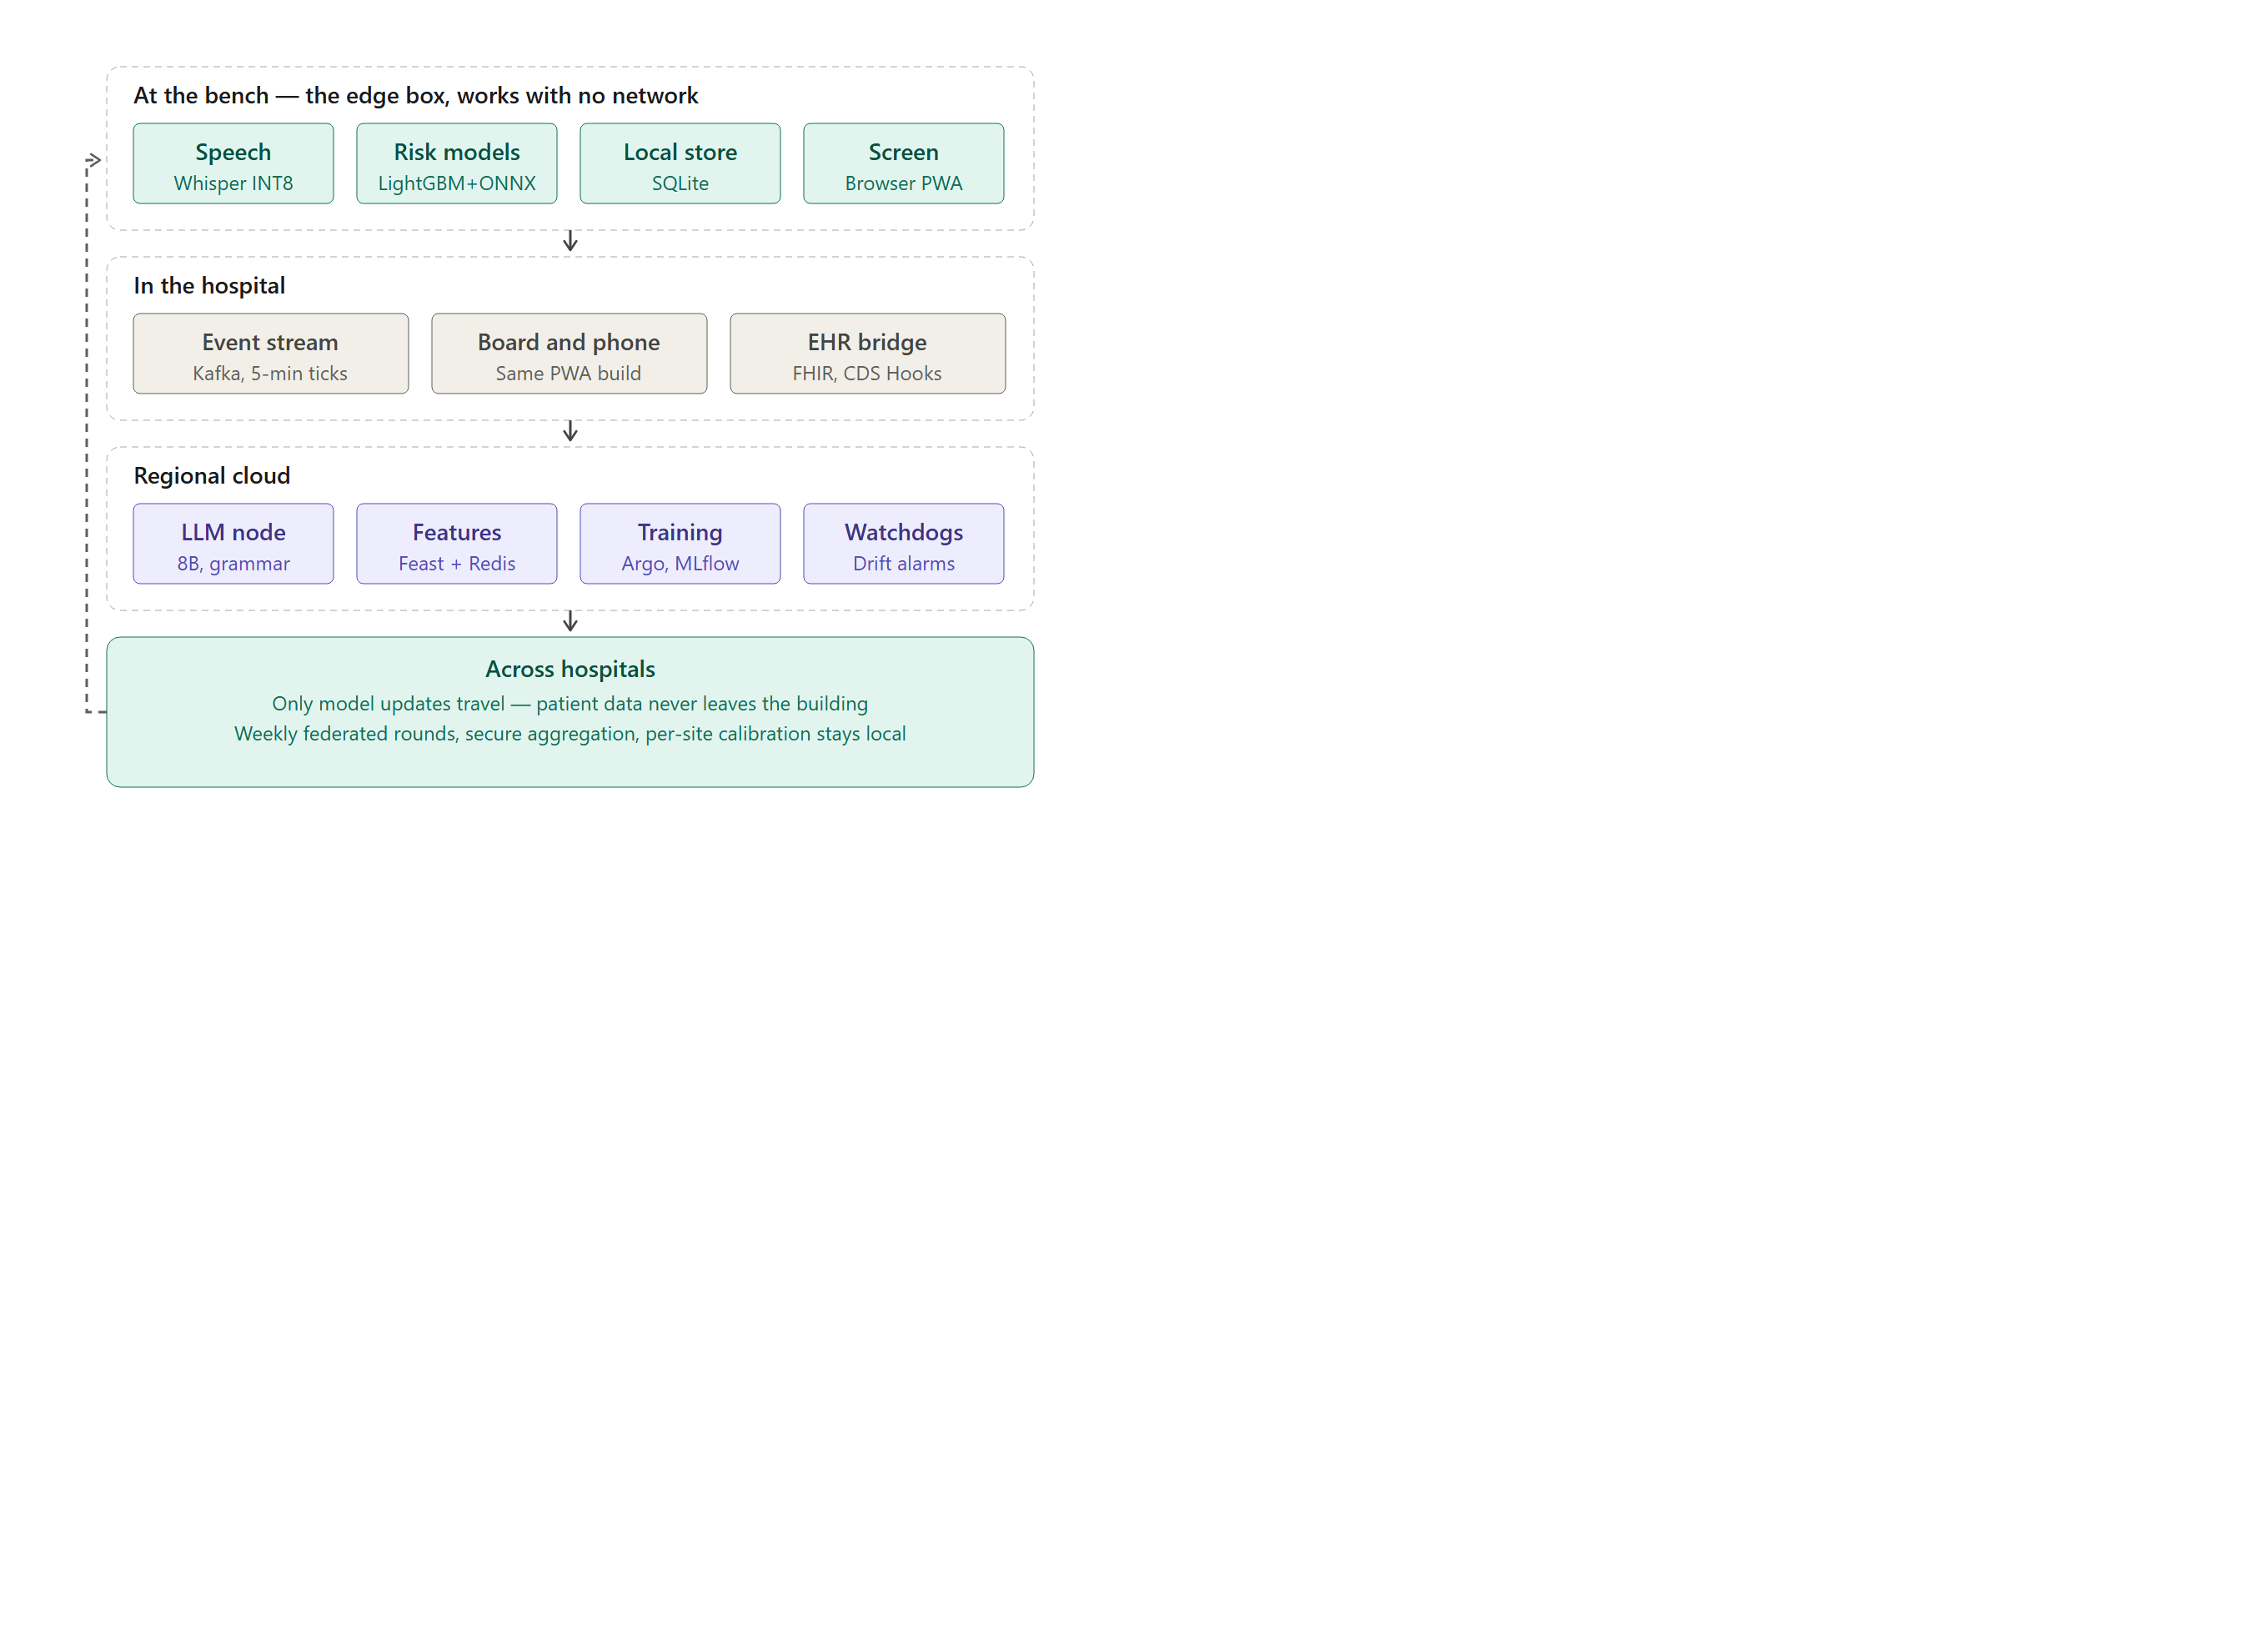
\includegraphics[width=\textwidth]{../diagrams/04-tech-stack-three-tiers.png}
    \caption{The Three-Tier Inference Hierarchy.}
\end{figure}

\section{Technology Stack \& Execution Constraints}
The system executes on commodity hardware, complying with the strict data locality mandates of the DPDP Act 2023. It explicitly bans mandatory dependencies on paid cloud GPU infrastructure.

\begin{itemize}
    \item \textbf{Frontend Interfaces:} Next.js 16, React 19, Tailwind CSS 4, utilizing native \texttt{webkitSpeechRecognition}.
    \item \textbf{Triage Orchestrator:} Python 3.10+, FastAPI, Uvicorn, Scikit-learn, Pandas.
    \item \textbf{Perception Models:} \texttt{faster-whisper} (CTranslate2, int8) and Llama.cpp for offline structural parsing.
\end{itemize}

\section{The Confined Role of the Large Language Model (LLM)}
The Large Language Model is strictly confined to \textbf{Track A (Perception Layer)}. 

\begin{figure}[ht]
    \centering
    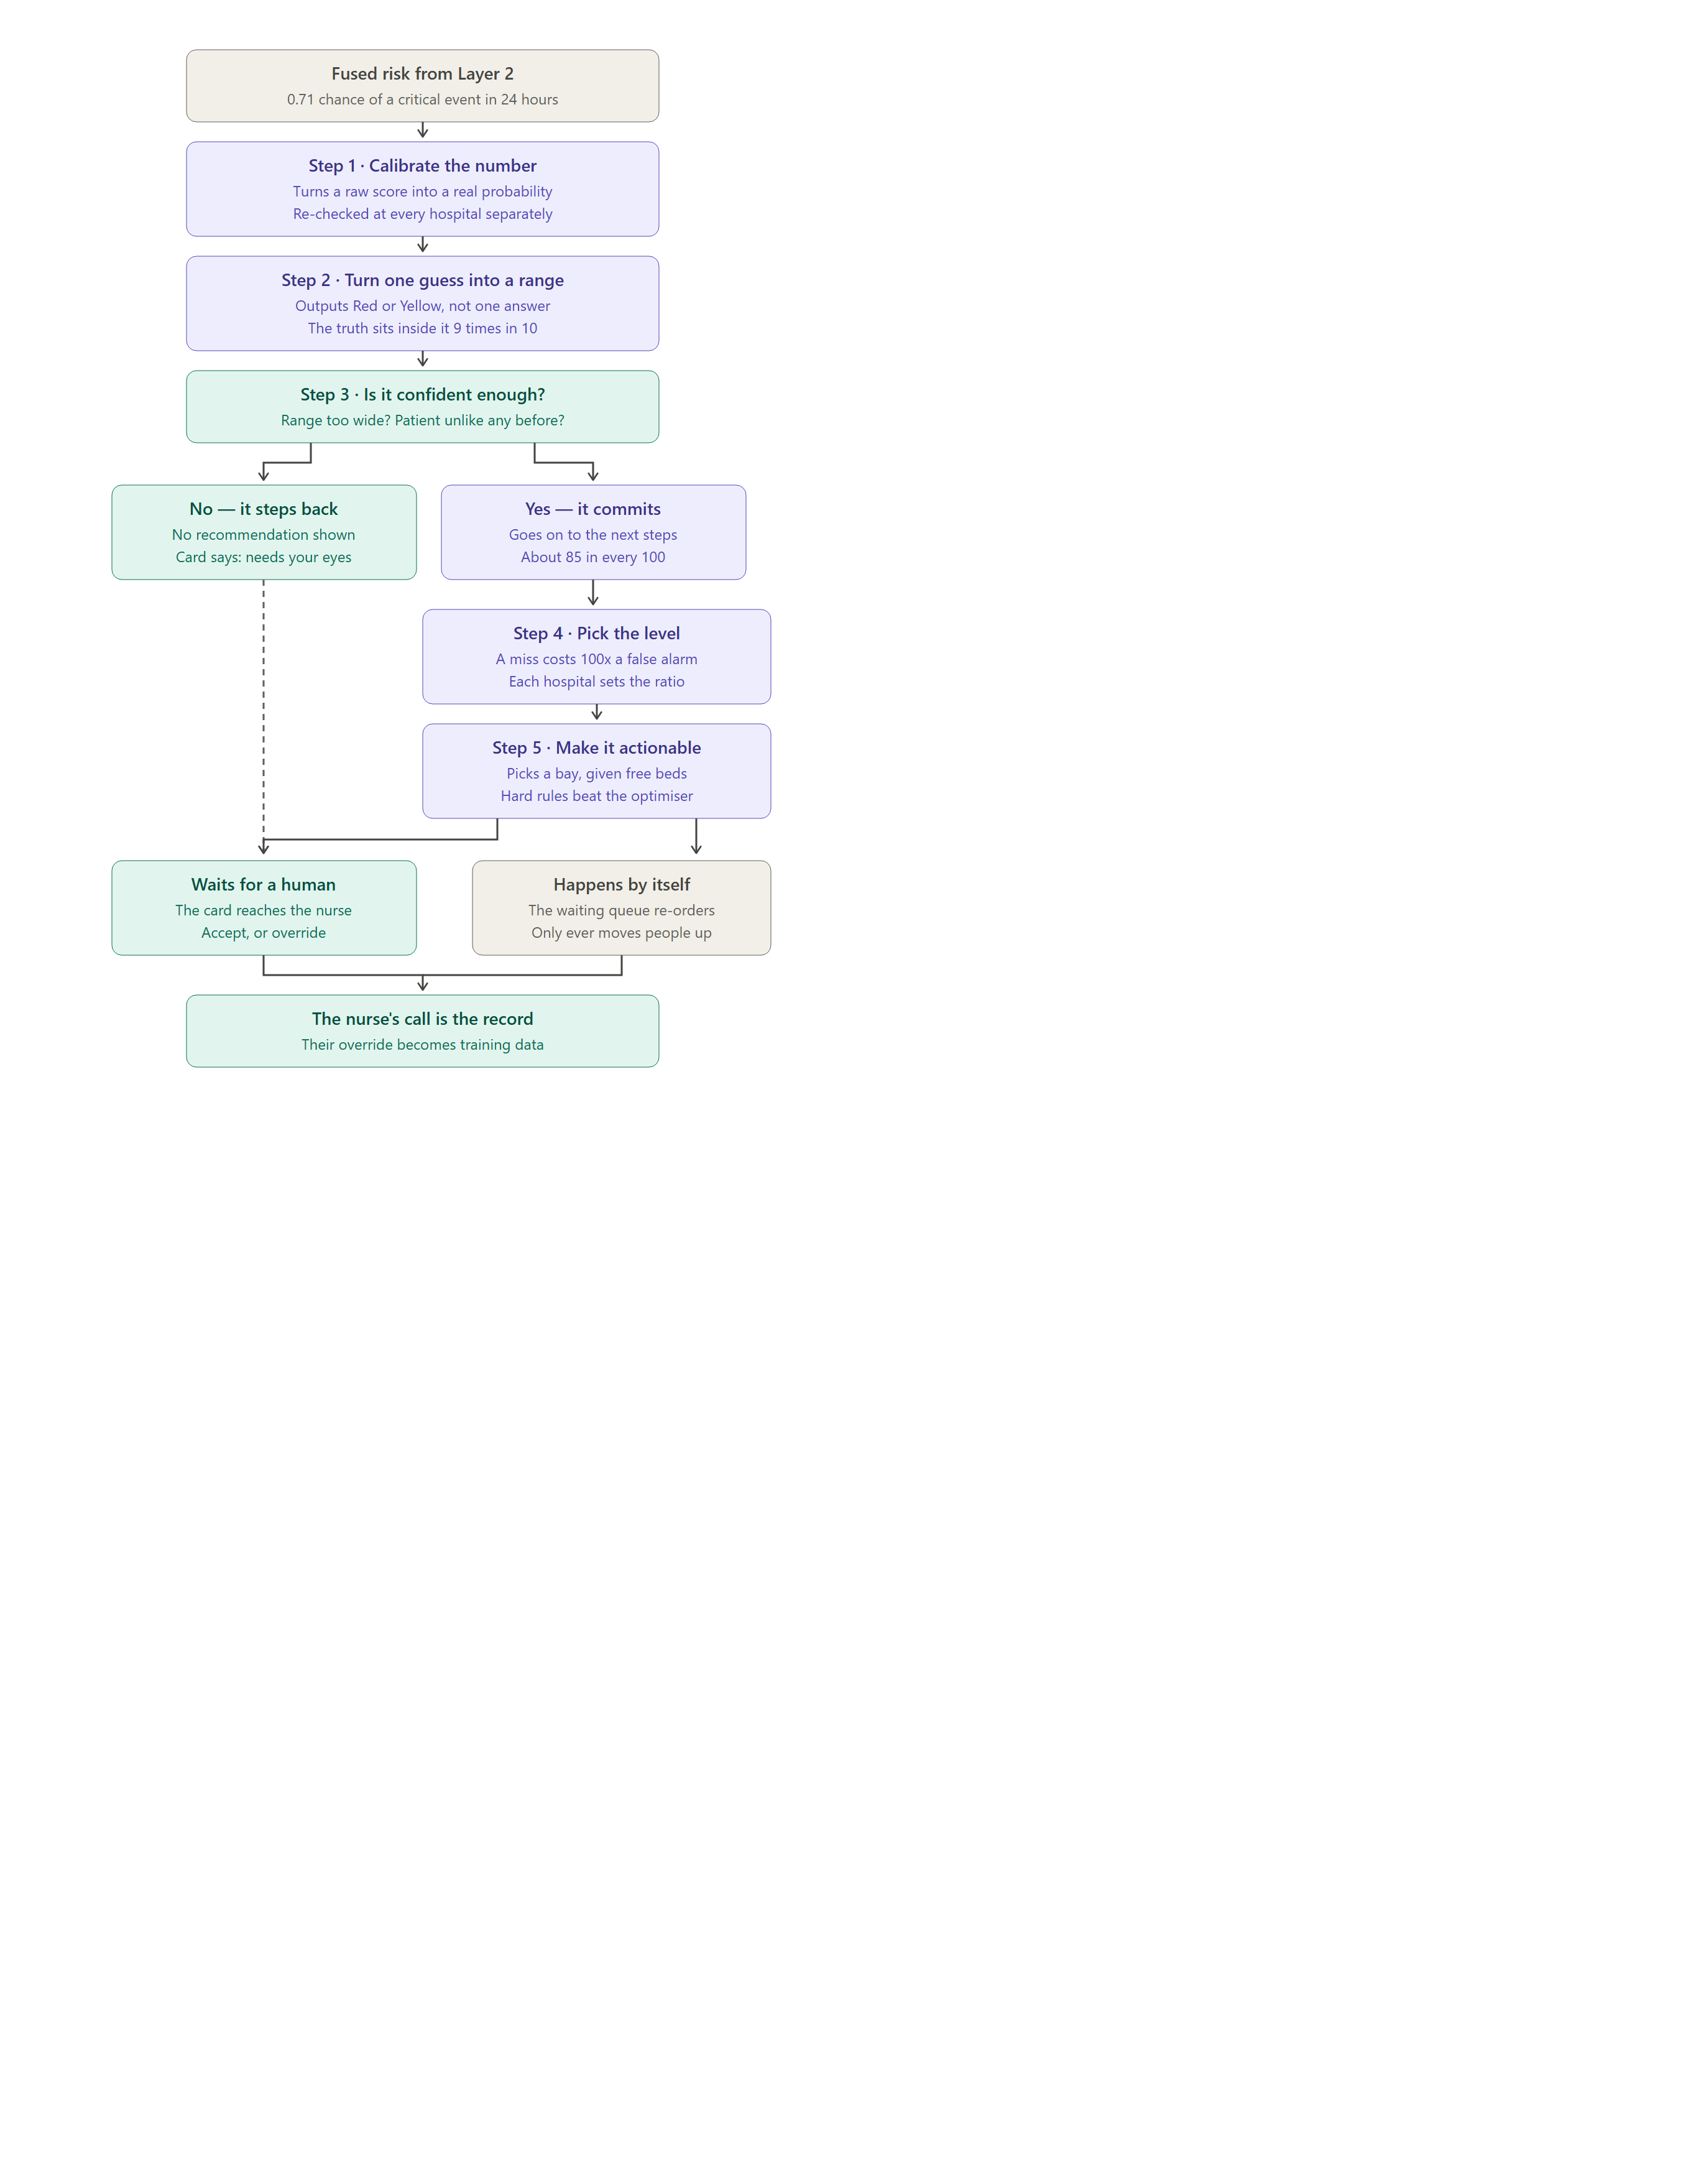
\includegraphics[width=\textwidth]{../diagrams/02-post-risk-engine-decision-path.png}
    \caption{The Semantic Boundary: The model reports, the rule evaluates.}
\end{figure}

The LLM operates purely as a structural parser, translating unstructured patient narrative into a rigid JSON schema. It is structurally prohibited from producing an acuity score, assigning a triage band, or issuing clinical judgments. Should inference resources become constrained or the model output violate the schema, the system falls back to a deterministic, keyword-based structurer. 

\section{Synthetic Data Production}
To validate the system's edge cases without exposing Patient Health Information (PHI), the demonstration corpus is entirely synthetic. The 20-record dataset (\texttt{web/lib/seed/corpus.ts}) is generated deterministically to test Wait-Ceiling breaches, Out-Of-Distribution (OOD) gates, and zero-history ABHA paths.

\section{Repository Integrity \& Structure}
The repository is structured to enforce the separation of concerns between the architectural tracks:

\vspace{0.5cm}
\begin{lstlisting}[language=bash, basicstyle=\small\ttfamily, backgroundcolor=\color{gray!10}]
.
|-- web/                    # Track B: Next.js frontend (kiosk, board)
|-- backend/                # Track C: Python FastAPI orchestrator 
|-- docs/                   # Documentation and whitepaper specifications
|   |-- paper/              # LaTeX source files
|   |-- diagrams/           # SVG and PNG architecture diagrams
|   \-- submission/         # Compiled PDFs for evaluation
|-- archive/                # Quarantined legacy code
\-- .migration/             # Hashes proving migration integrity
\end{lstlisting}

\end{document}
